\begin{figure*}[!ht]
\center
%input
\centering
\begin{tabular}{p{0.13\linewidth}p{0.163\linewidth}p{0.163\linewidth}p{0.163\linewidth}p{0.163\linewidth}}
\centering{\textbf{Shape/Interest point}} & \centering Mini & \centering Bearing & \centering Knob & \centering Bracket 
\end{tabular}
\subfloat{ 
\label{fig:mvs:input}
\makebox[0.15\linewidth]{\raisebox{0.07\linewidth}{(a) Input point clouds}}
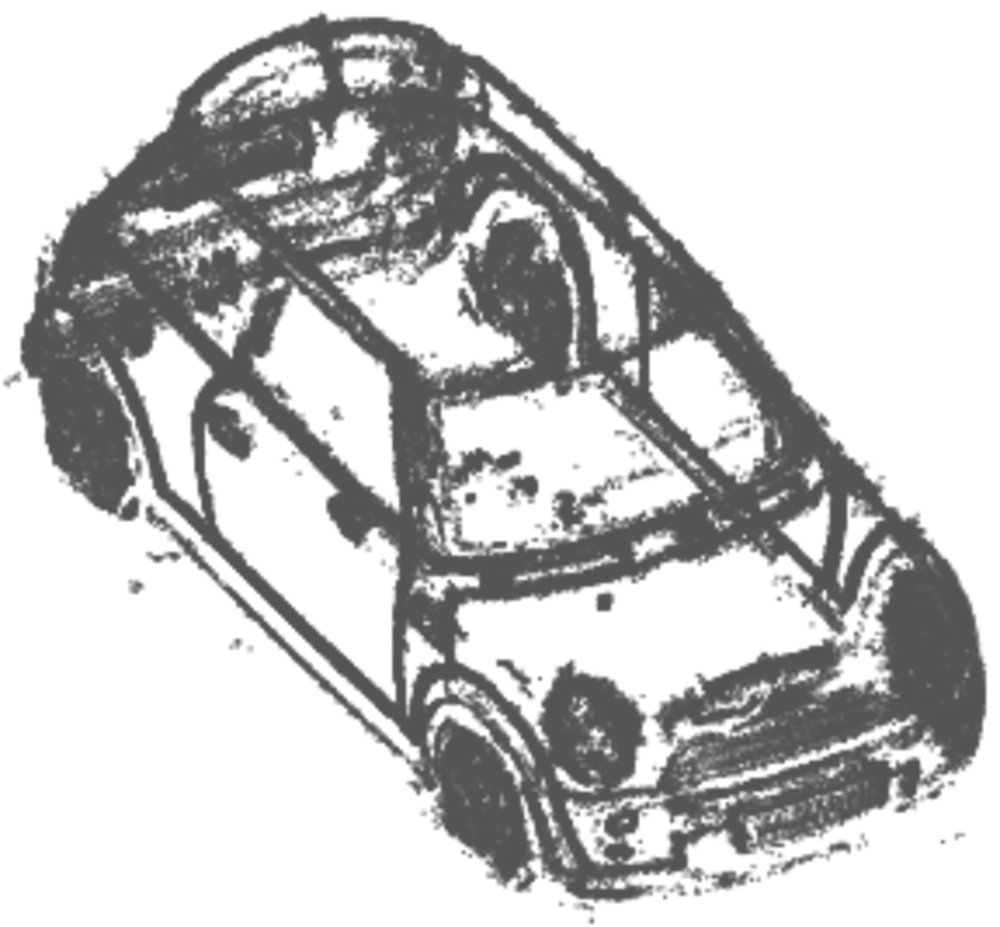
\includegraphics[width=0.175\linewidth]{./fig/eval/mini_input.jpg} \hspace{0mm}
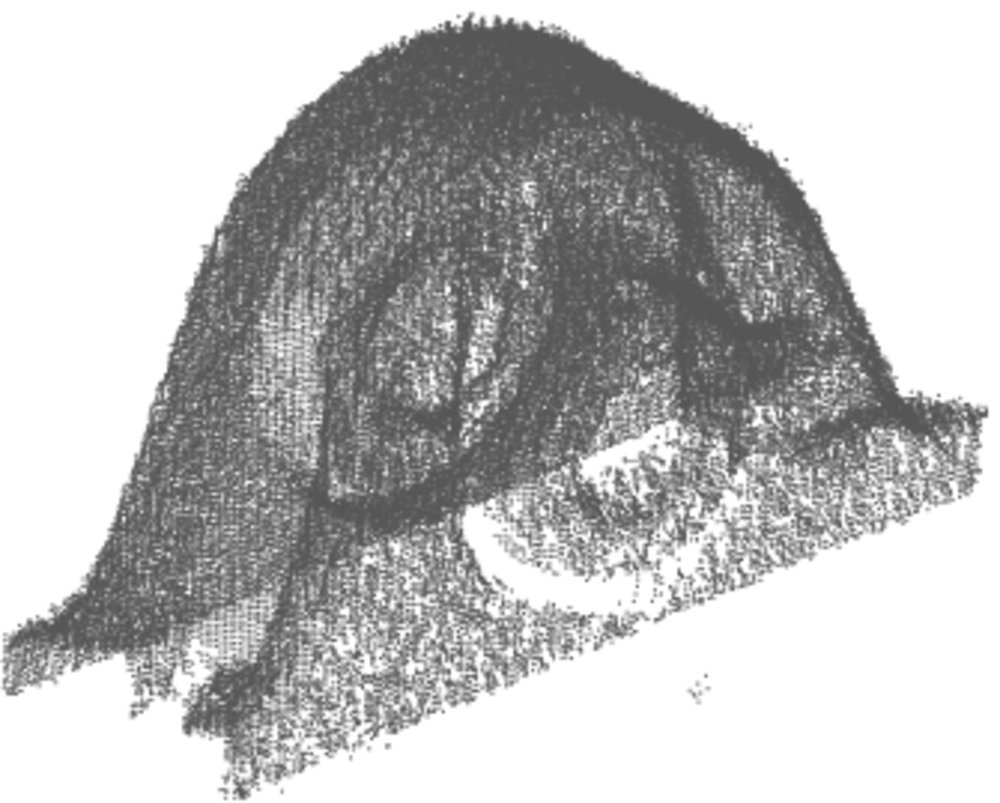
\includegraphics[width=0.175\linewidth]{./fig/eval/bearing_input.jpg}  \hspace{0mm} 
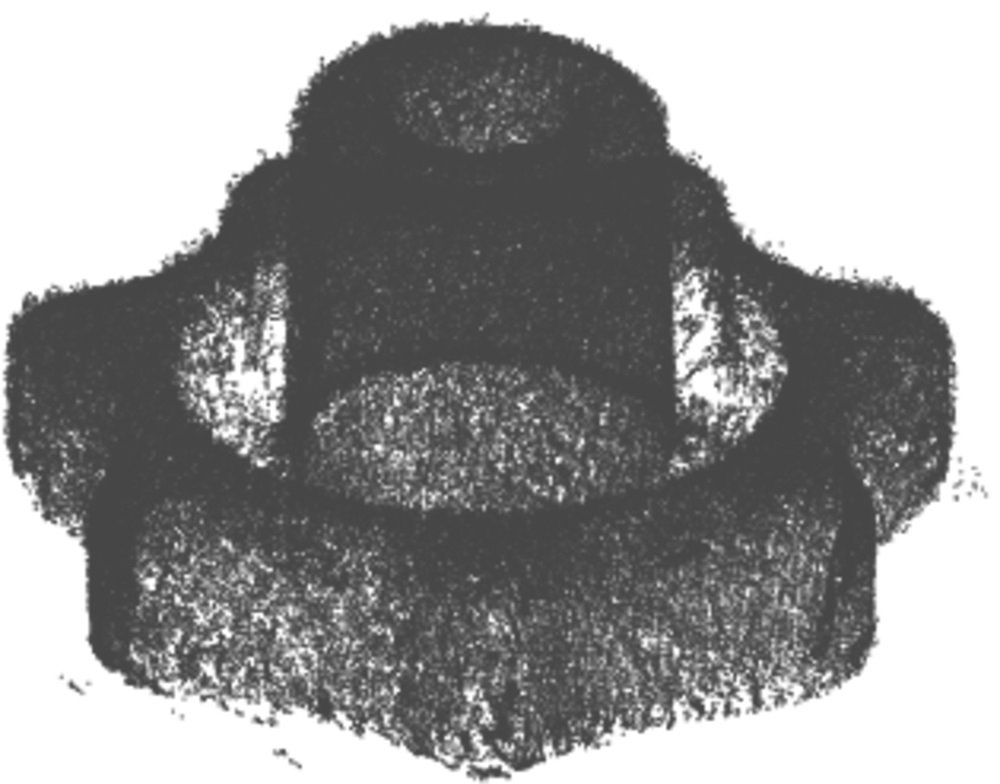
\includegraphics[width=0.175\linewidth]{./fig/eval/knob_input.jpg} \hspace{0mm} 
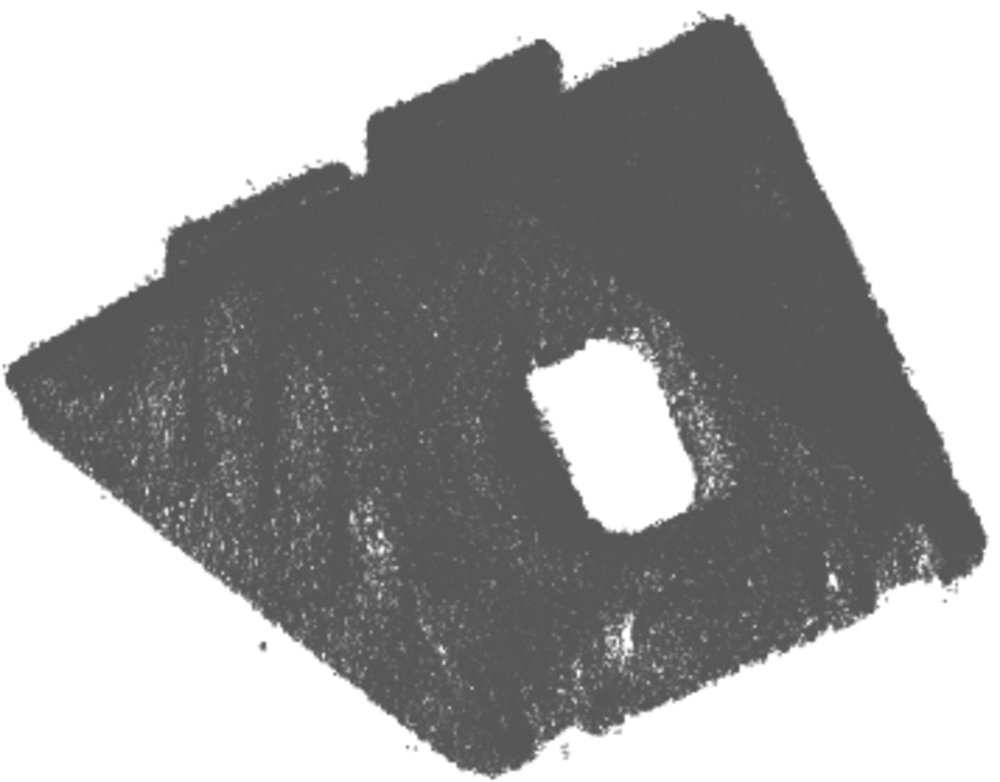
\includegraphics[width=0.175\linewidth]{./fig/eval/bracket_input.jpg} 
} \vspace{-4.4mm} 
\\ 
% DoG
\subfloat{ 
\label{fig:mvs:dog}
\makebox[0.15\linewidth]{\raisebox{0.07\linewidth}{(b) DoG}}
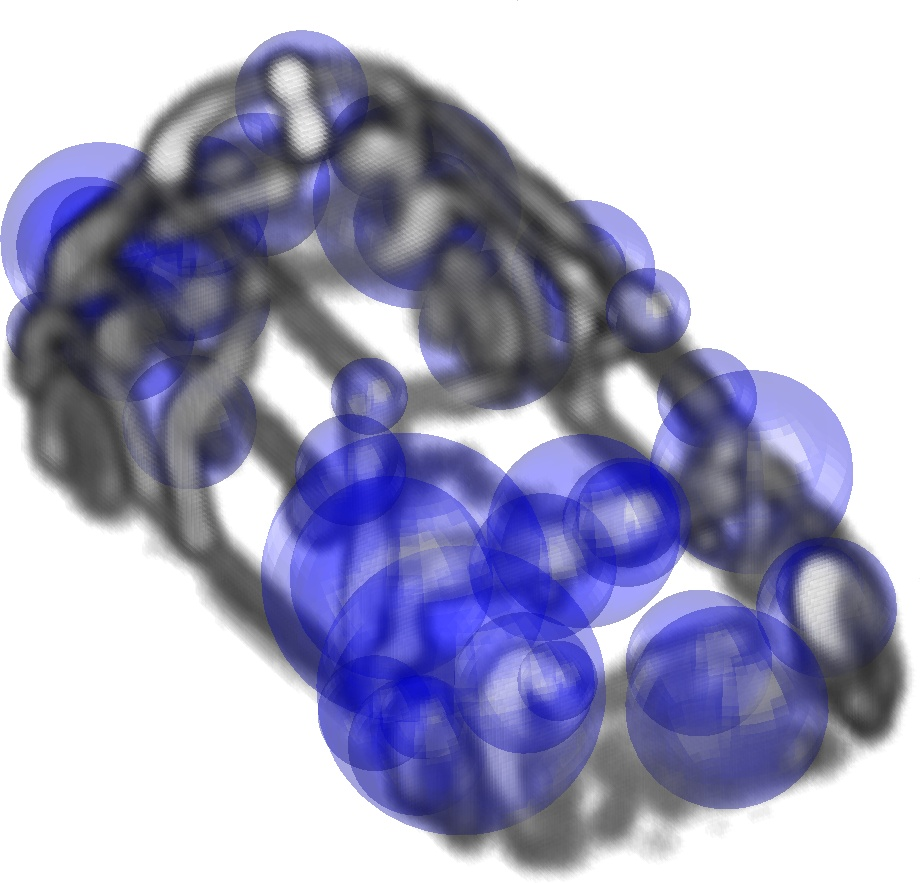
\includegraphics[width=0.175\linewidth]{./fig/eval/mini_dog.jpg} \hspace{0mm} 
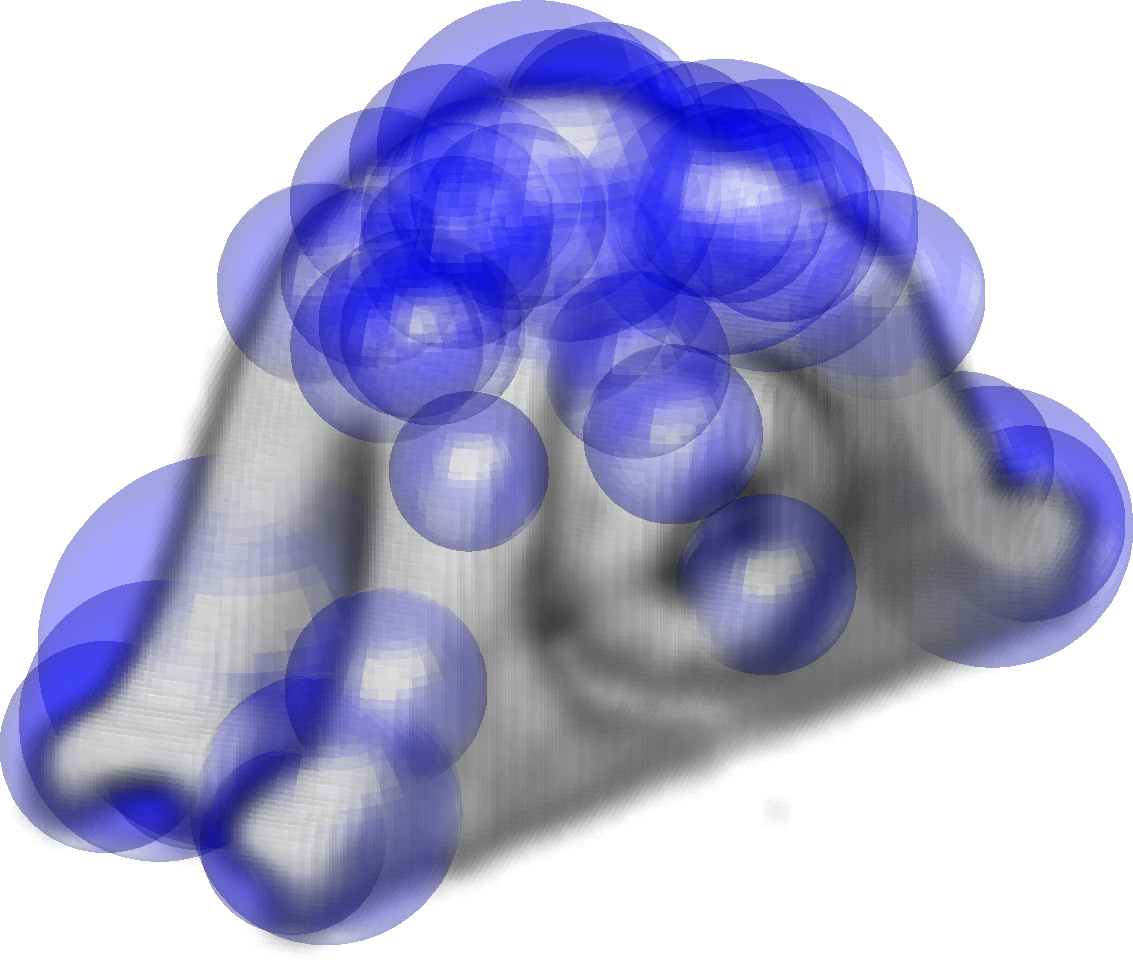
\includegraphics[width=0.175\linewidth]{./fig/eval/bearing_dog.jpg}  \hspace{0mm} 
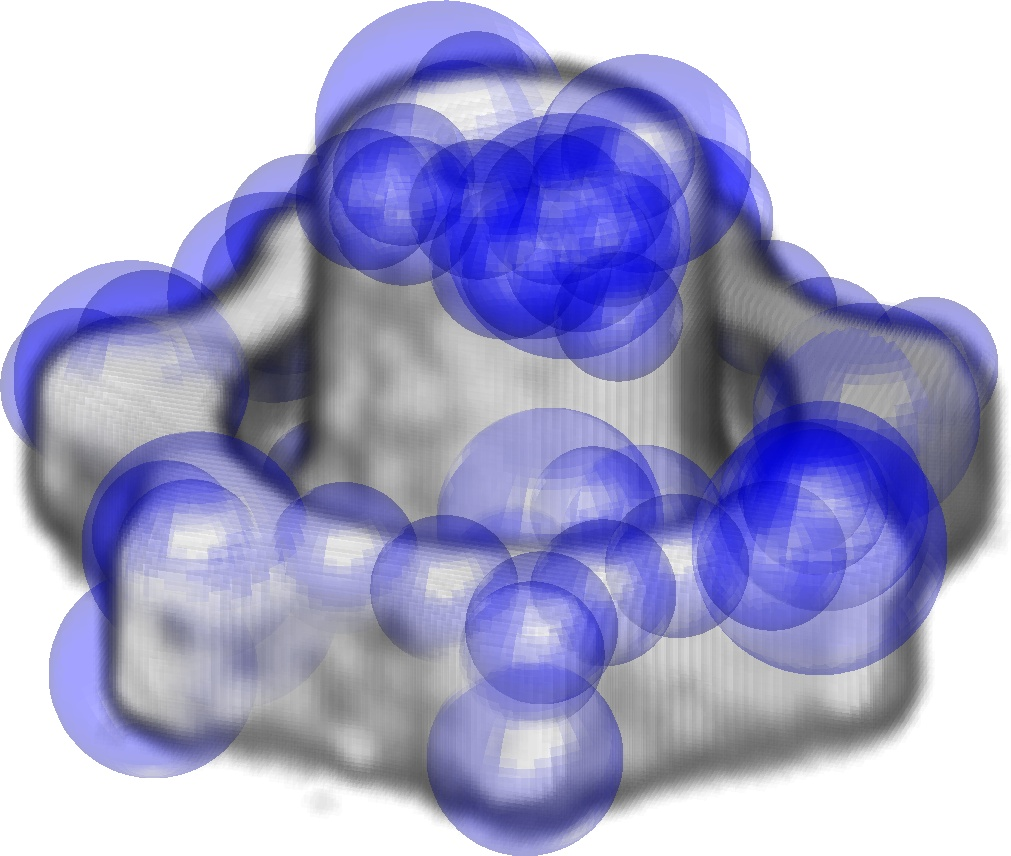
\includegraphics[width=0.175\linewidth]{./fig/eval/knob_dog.jpg} \hspace{0mm}
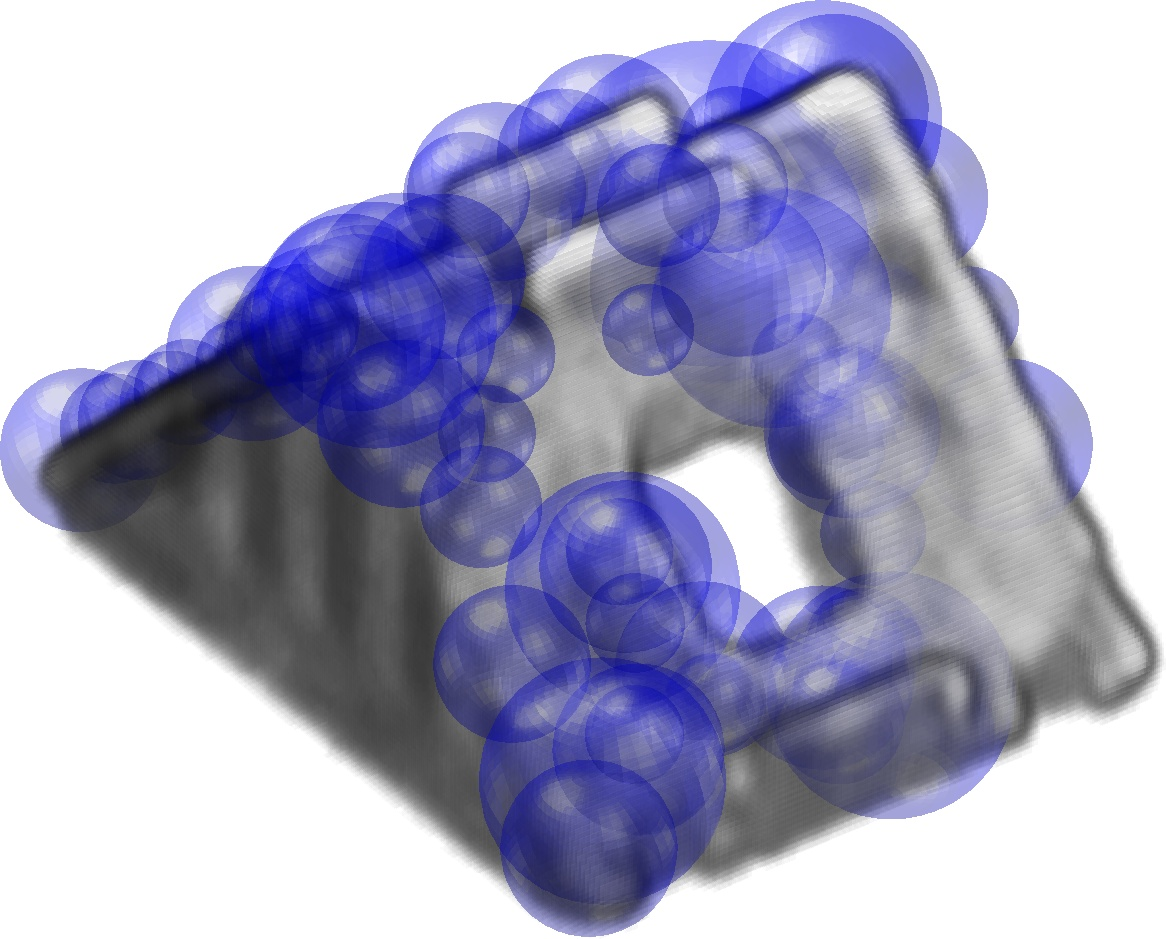
\includegraphics[width=0.175\linewidth]{./fig/eval/bracket_dog.jpg} 
} \vspace{-4.4mm} 
\\ 
% SURF 
\subfloat{ 
\label{fig:mvs:surf}
\makebox[0.15\linewidth]{\raisebox{0.07\linewidth}{(c) SURF}}
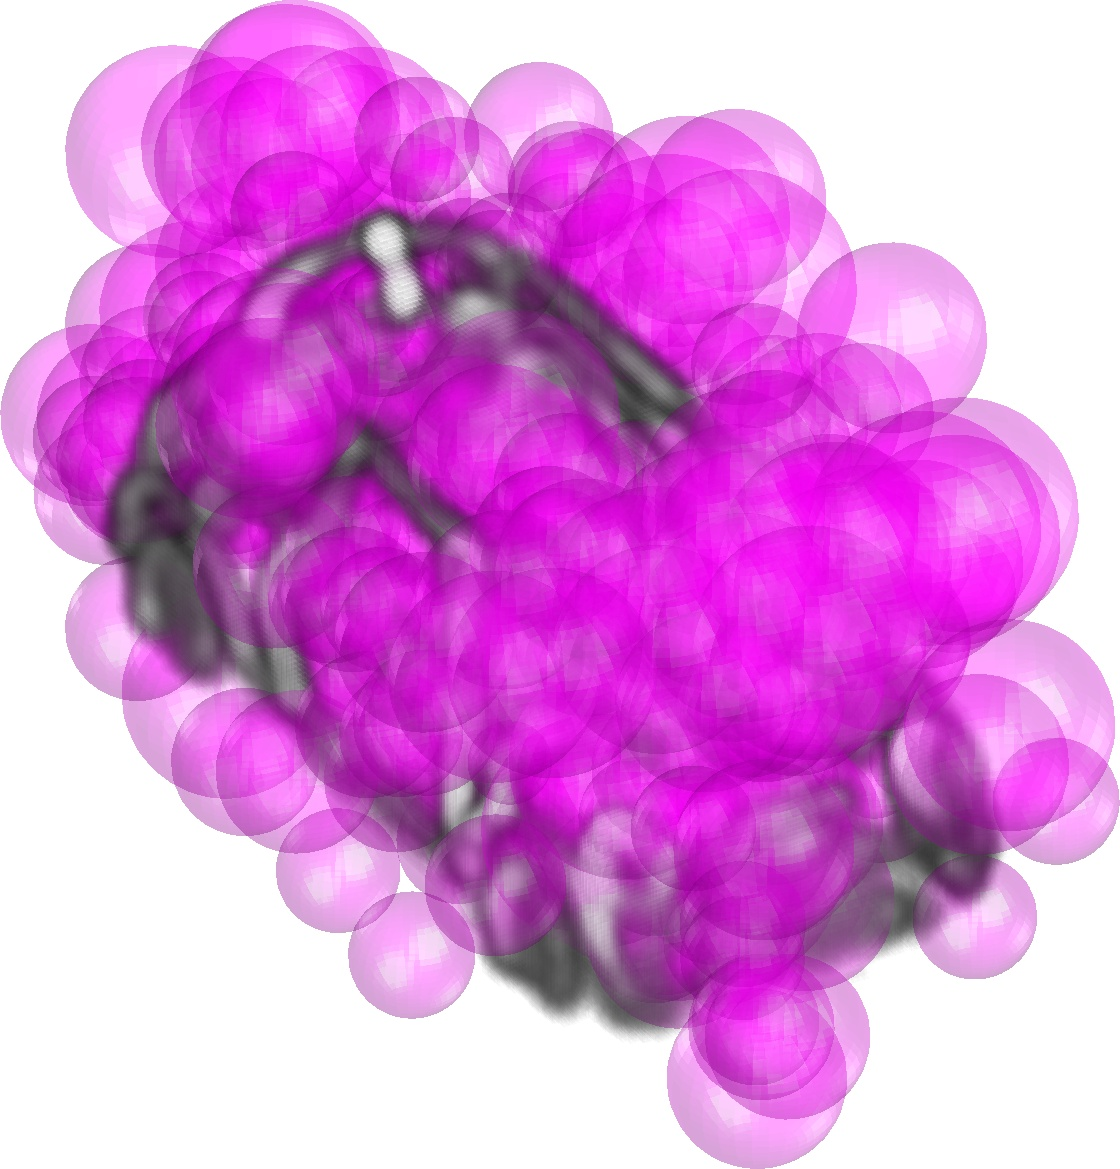
\includegraphics[width=0.175\linewidth]{./fig/eval/mini_surf.jpg} \hspace{0mm}
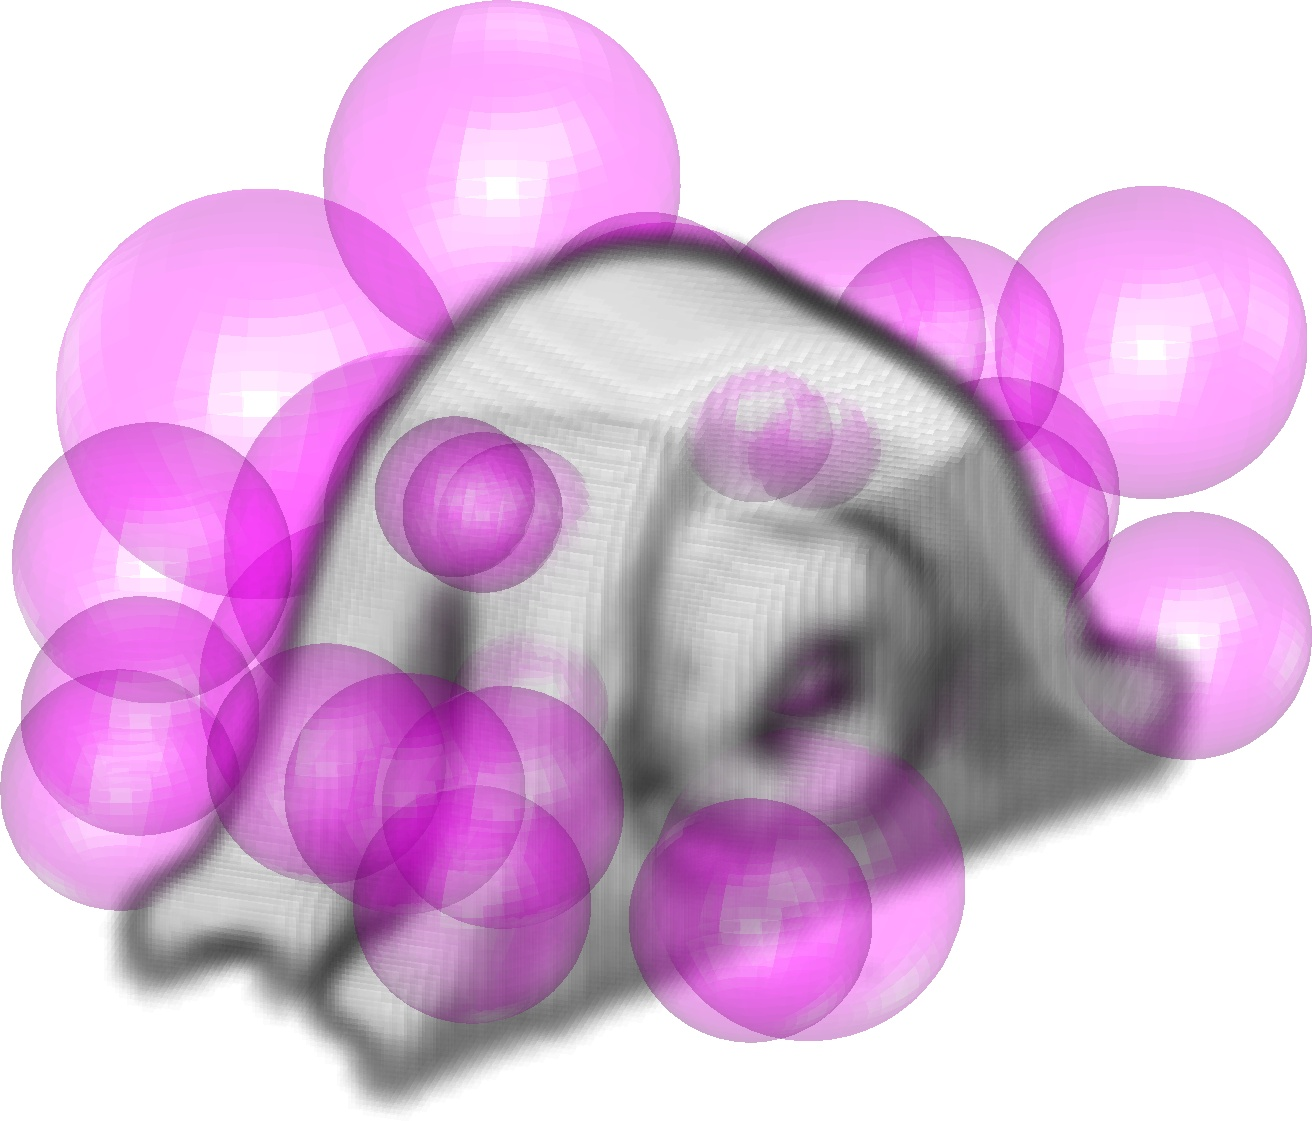
\includegraphics[width=0.175\linewidth]{./fig/eval/bearing_surf.jpg}  \hspace{0mm} 
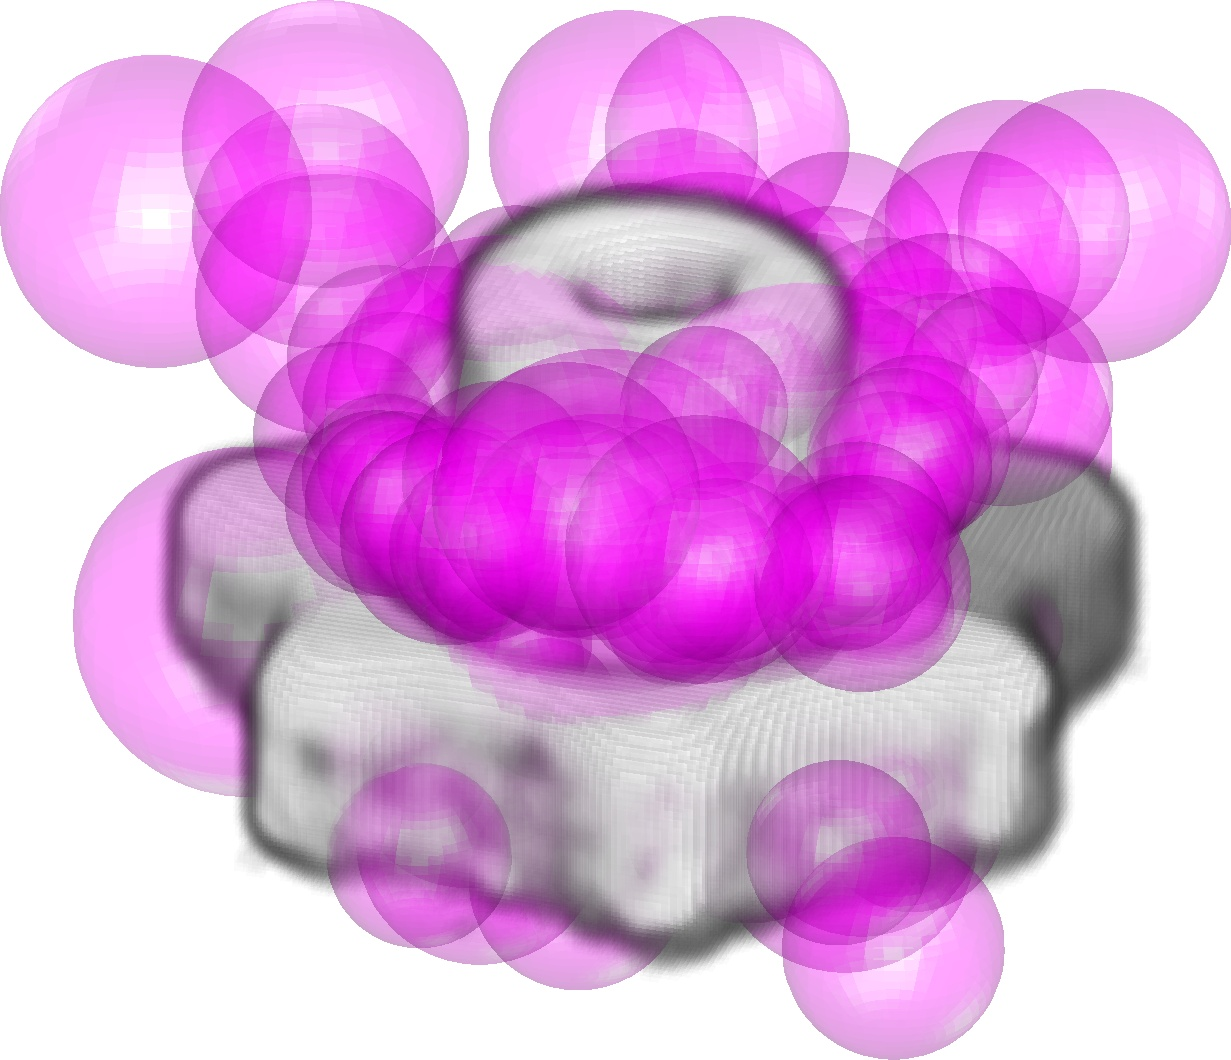
\includegraphics[width=0.175\linewidth]{./fig/eval/knob_surf.jpg} \hspace{0mm}
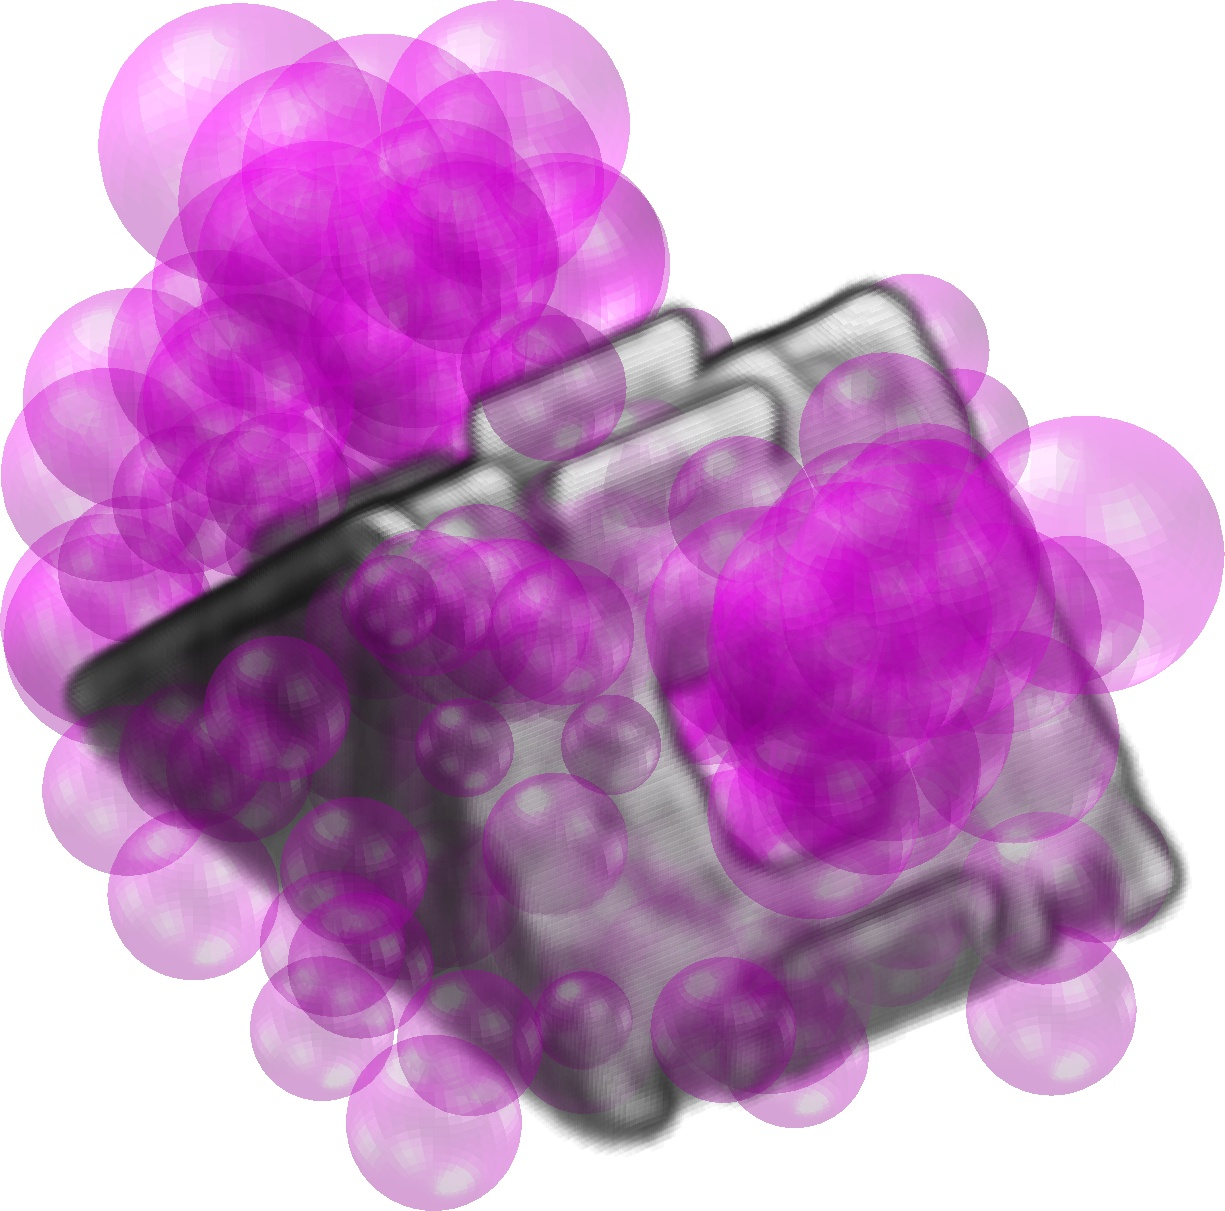
\includegraphics[width=0.175\linewidth]{./fig/eval/bracket_surf.jpg} 
} \vspace{-4.4mm}
\\
% HARRIS
\subfloat{ 
\label{fig:mvs:harris}
\makebox[0.15\linewidth]{\raisebox{0.07\linewidth}{(d) Harris}} 
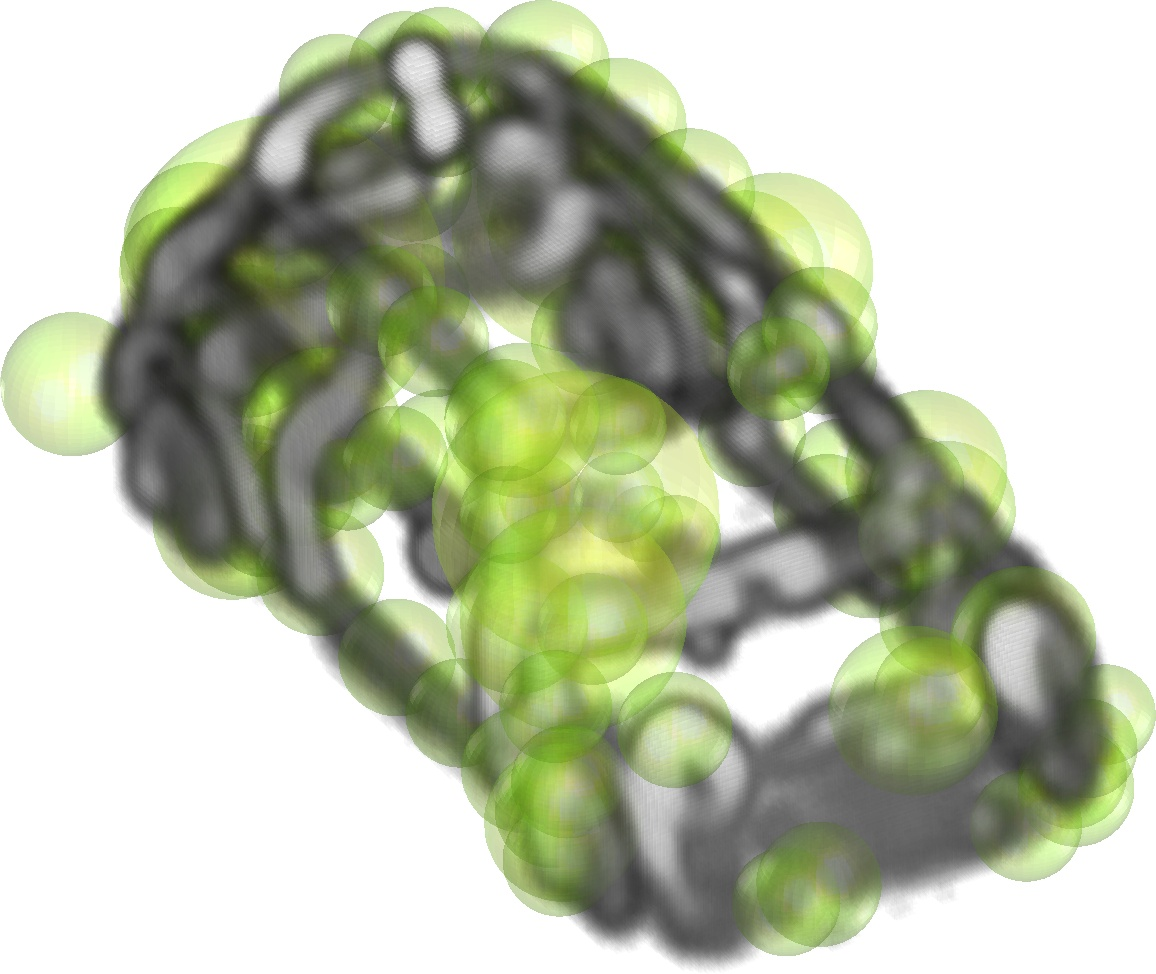
\includegraphics[width=0.175\linewidth]{./fig/eval/mini_harris.jpg} \hspace{0mm}
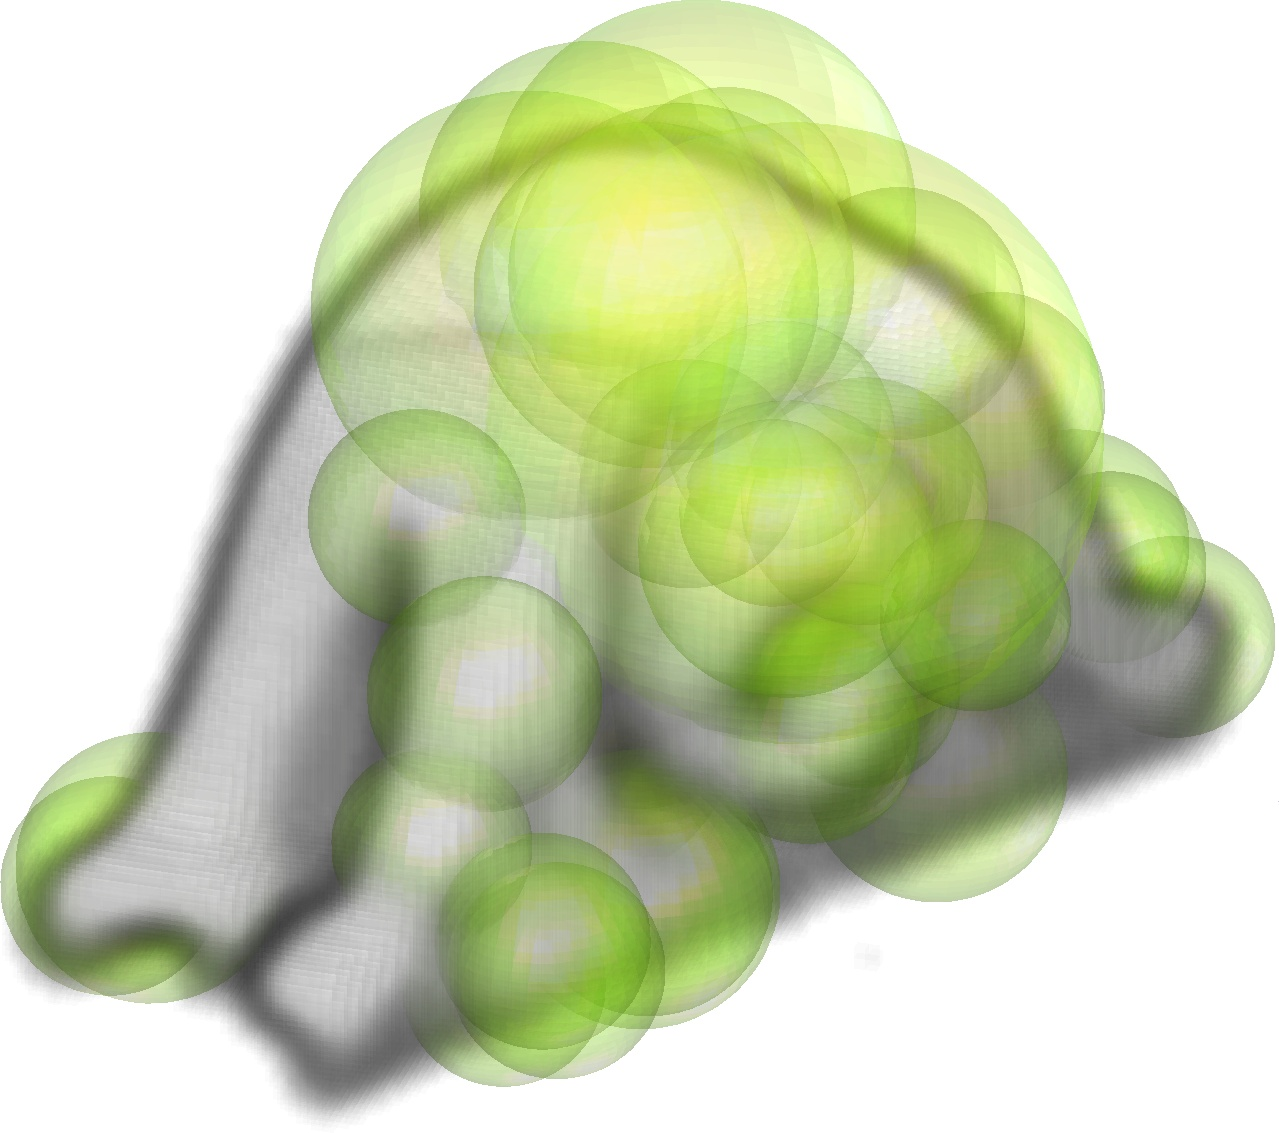
\includegraphics[width=0.175\linewidth]{./fig/eval/bearing_harris.jpg}  \hspace{0mm}
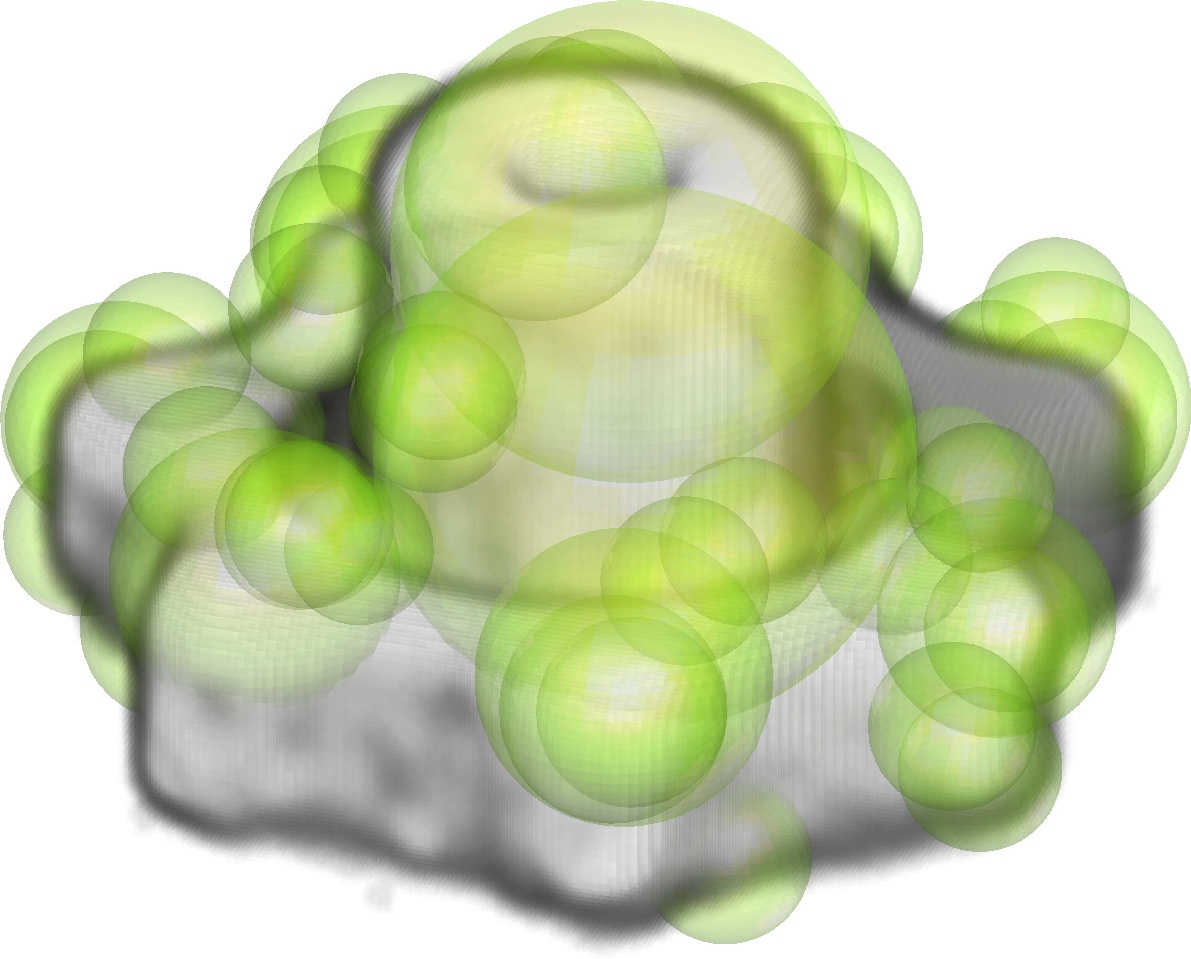
\includegraphics[width=0.175\linewidth]{./fig/eval/knob_harris.jpg} \hspace{0mm}
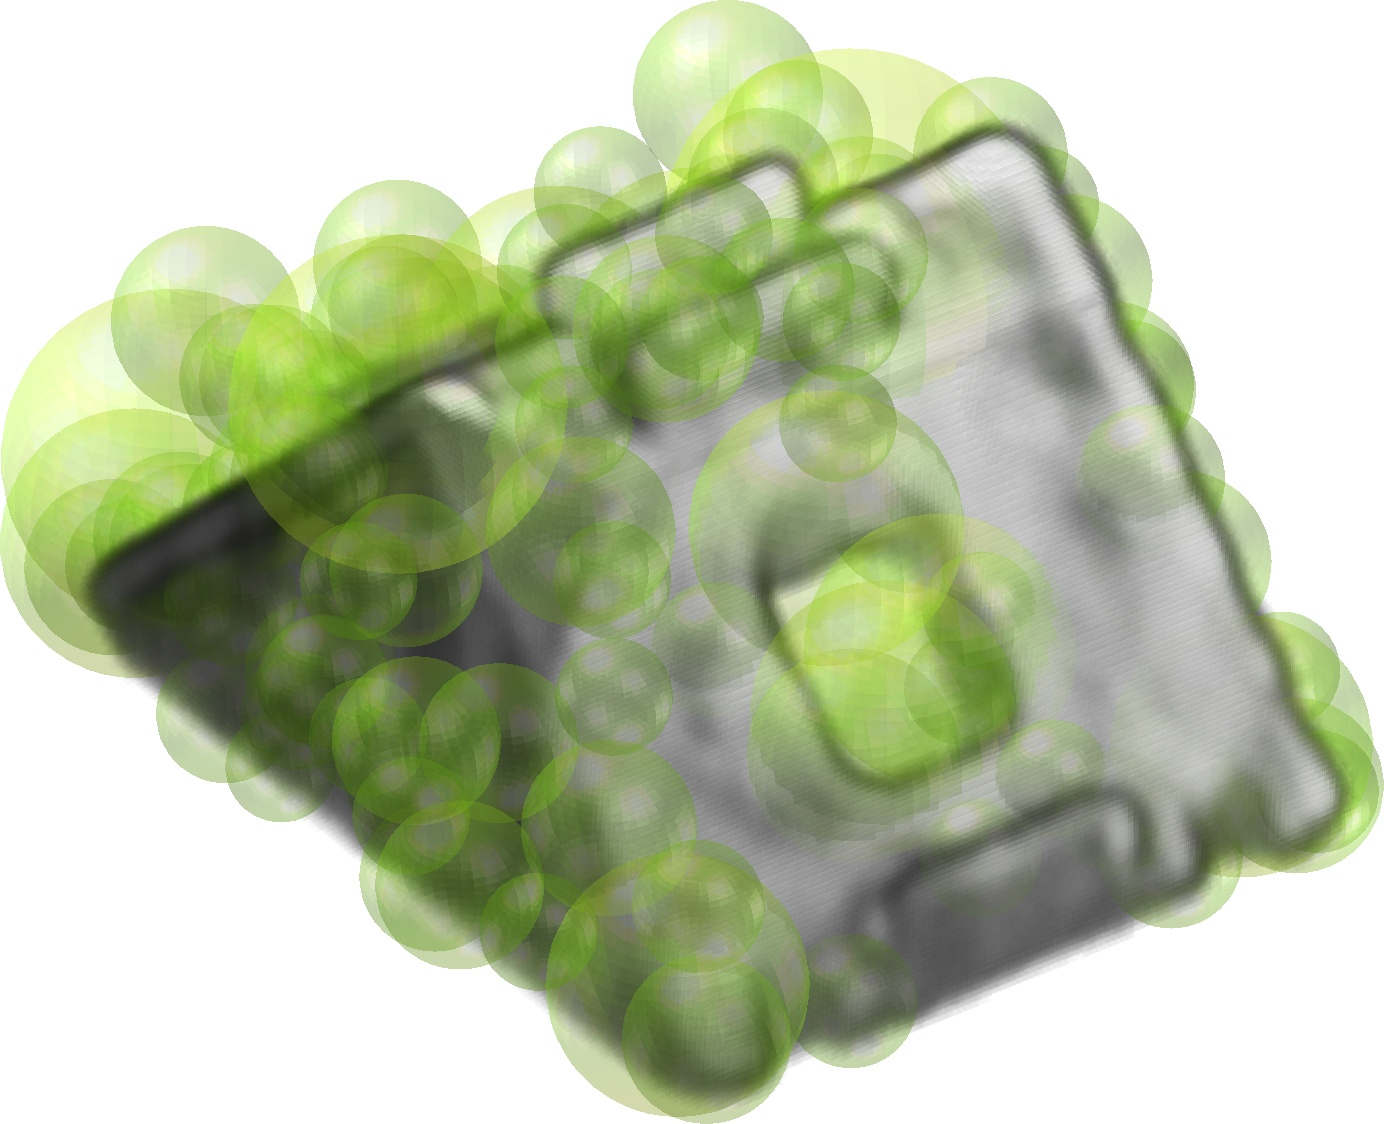
\includegraphics[width=0.175\linewidth]{./fig/eval/bracket_harris.jpg} 
} \vspace{-4.4mm}
\\
% HESSIAN
\subfloat{ 
\label{fig:mvs:hessian}
\makebox[0.15\linewidth]{\raisebox{0.07\linewidth}{(e) DoH}}
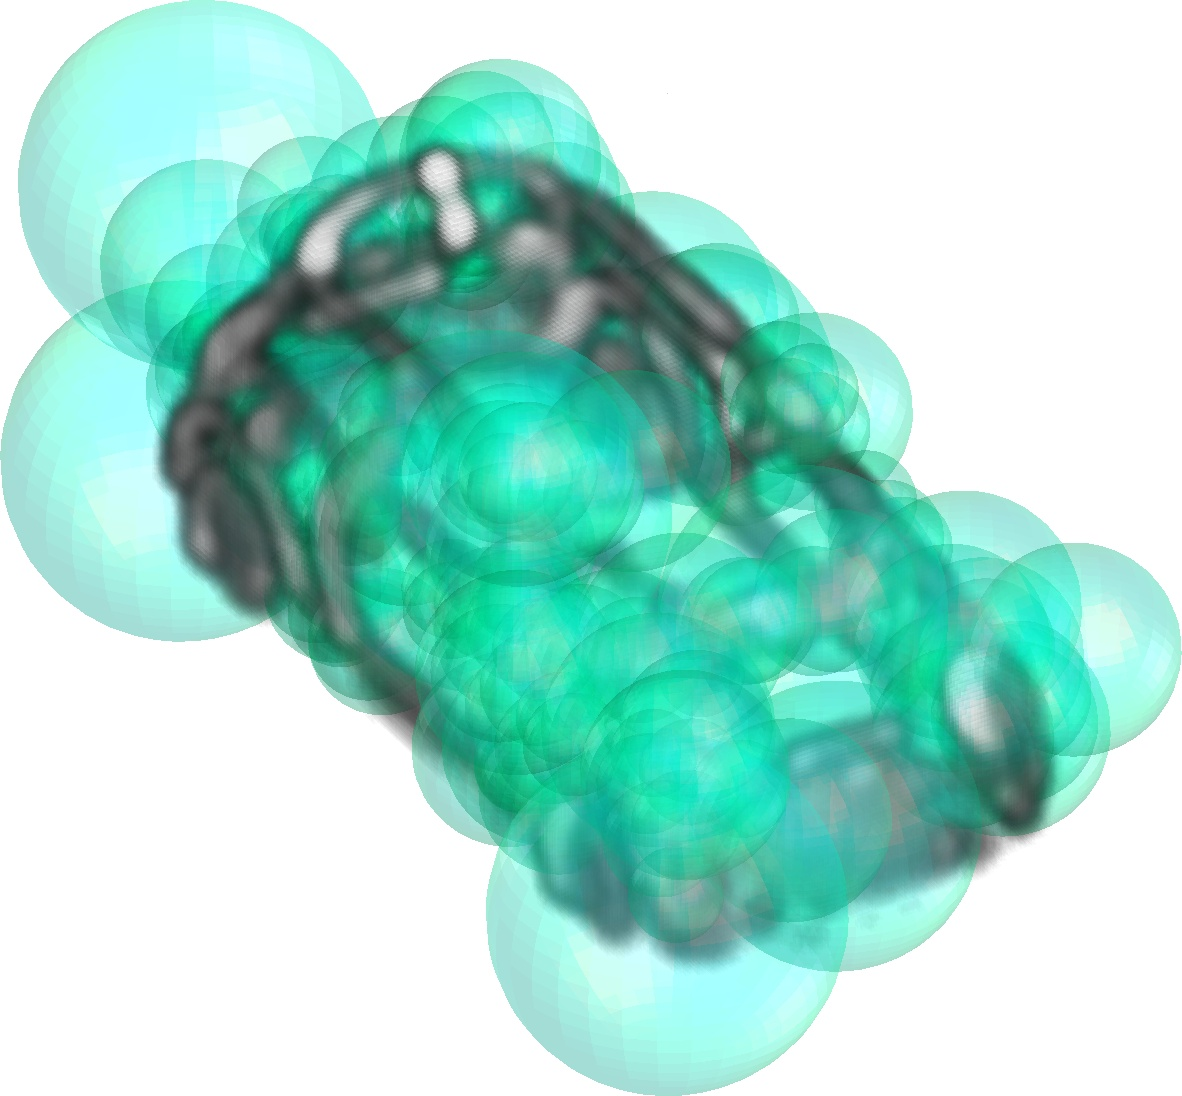
\includegraphics[width=0.175\linewidth]{./fig/eval/mini_hessian.jpg} \hspace{0mm}
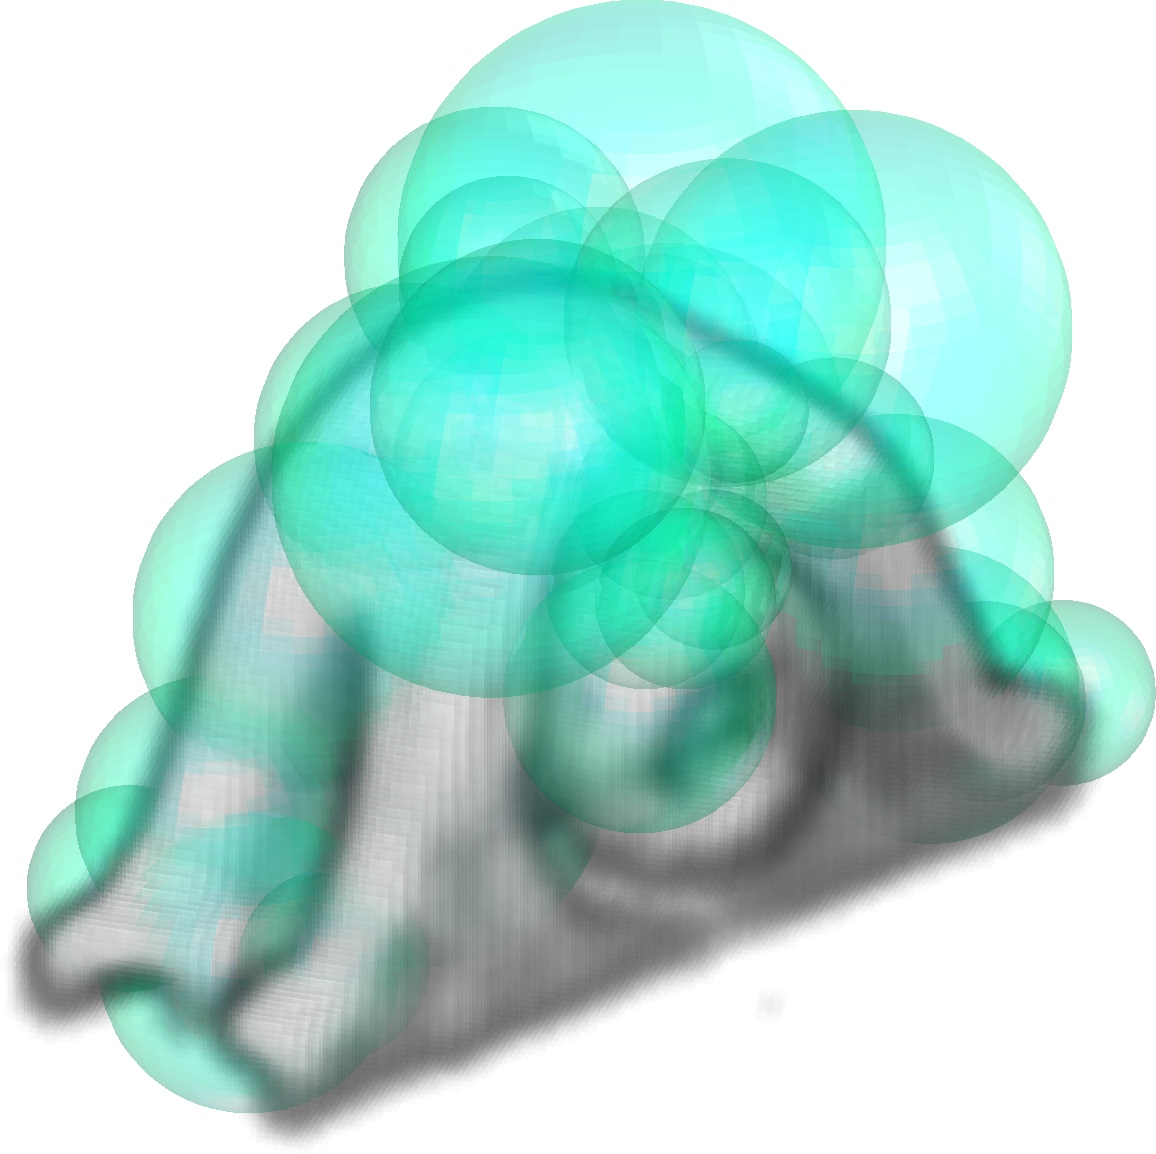
\includegraphics[width=0.175\linewidth]{./fig/eval/bearing_hessian.jpg}  \hspace{0mm} 
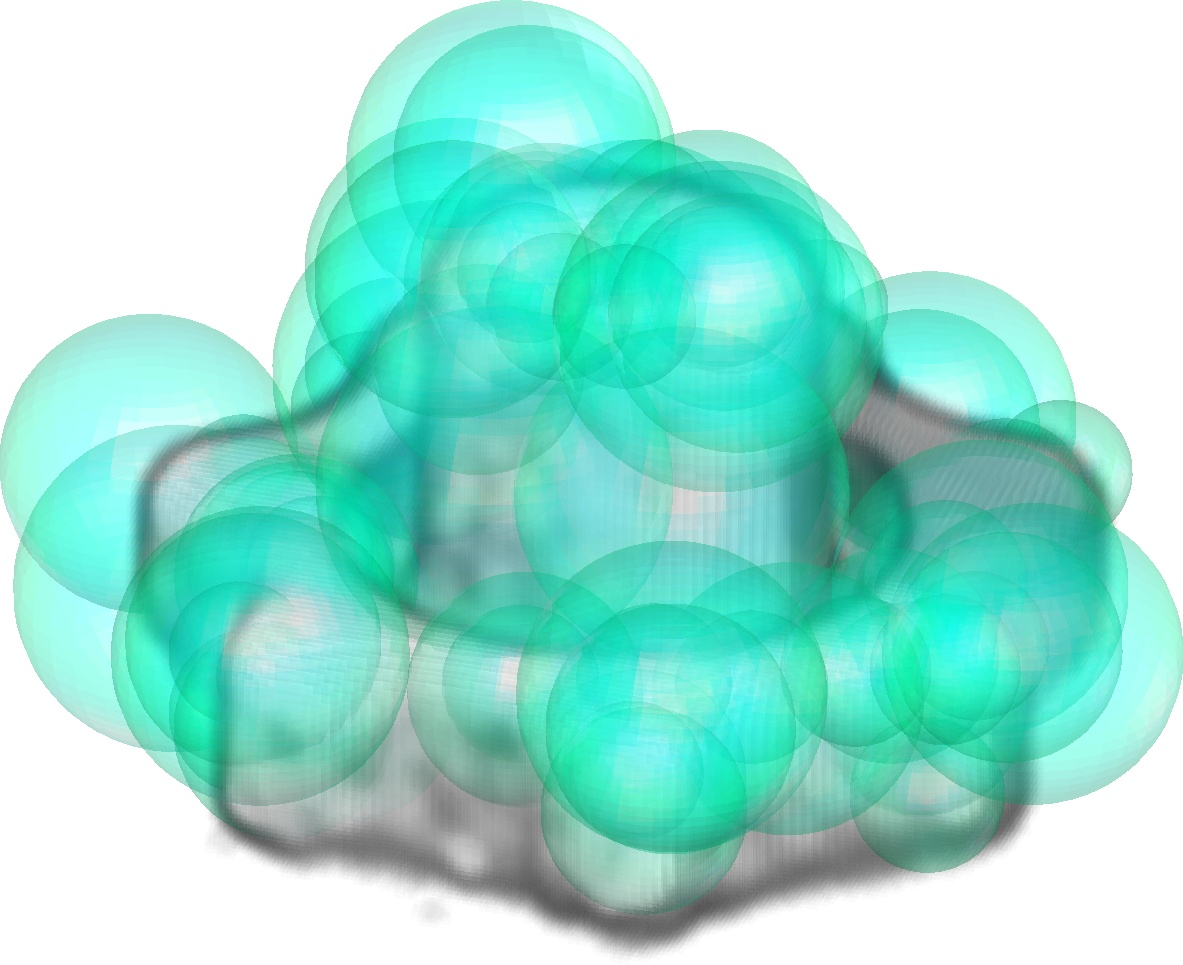
\includegraphics[width=0.175\linewidth]{./fig/eval/knob_hessian.jpg} \hspace{0mm}
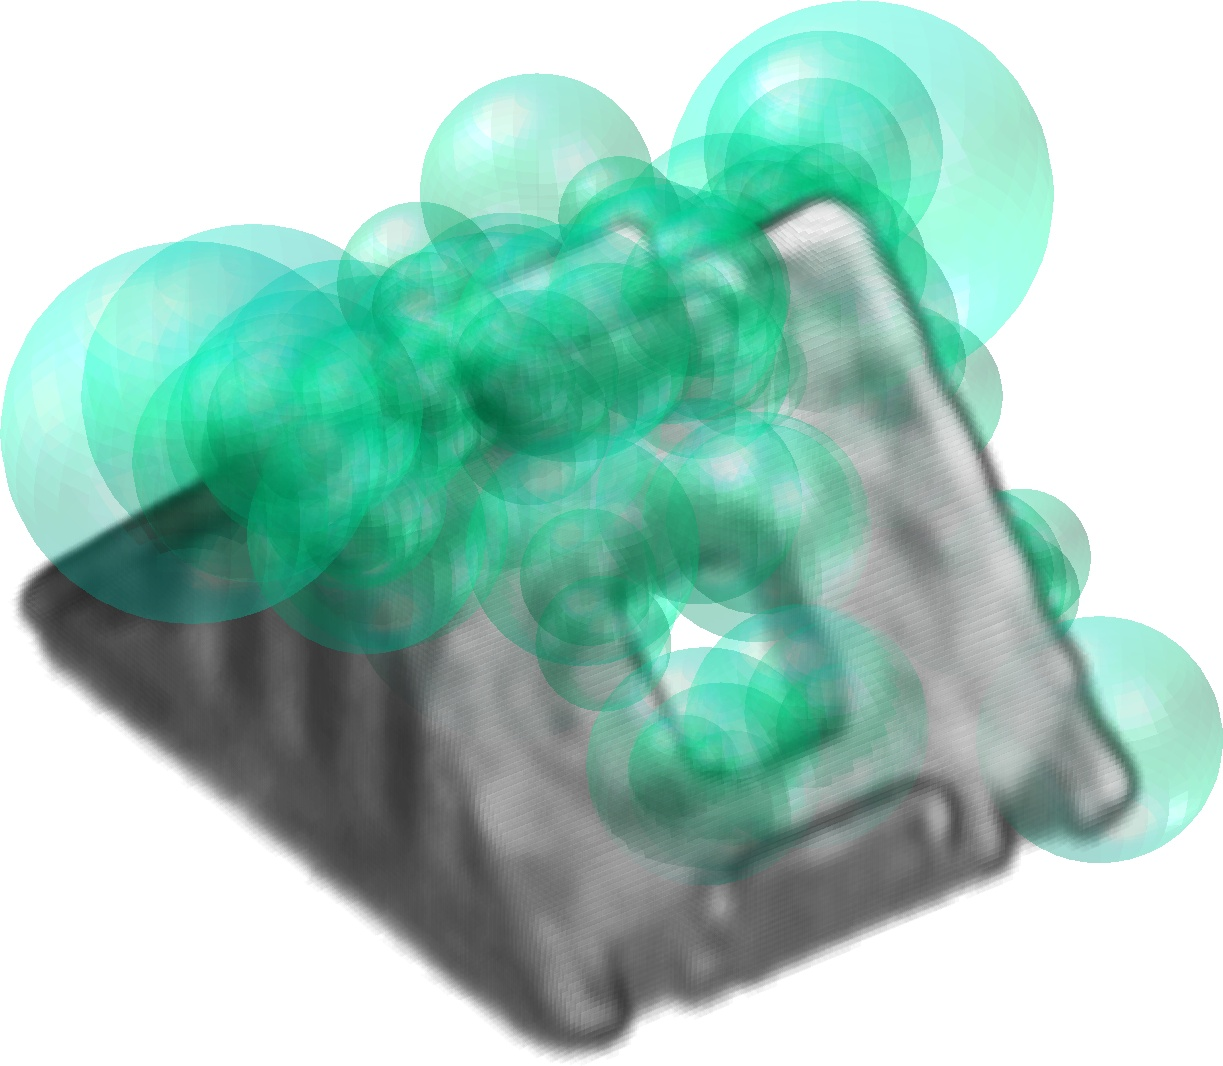
\includegraphics[width=0.175\linewidth]{./fig/eval/bracket_hessian.jpg} 
} \vspace{-4.4mm}
\\
% FAST
\subfloat{ 
\label{fig:mvs:fast}
\makebox[0.15\linewidth]{\raisebox{0.07\linewidth}{(f) V-FAST}}
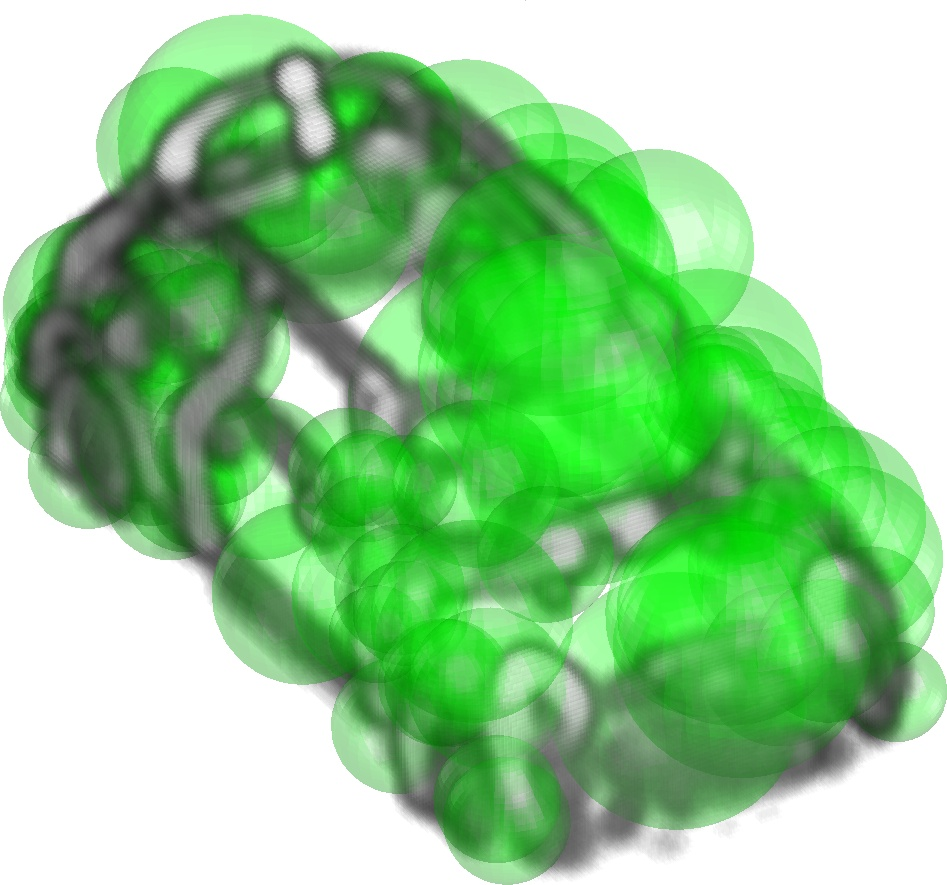
\includegraphics[width=0.175\linewidth]{./fig/eval/mini_fast.jpg} \hspace{0mm}
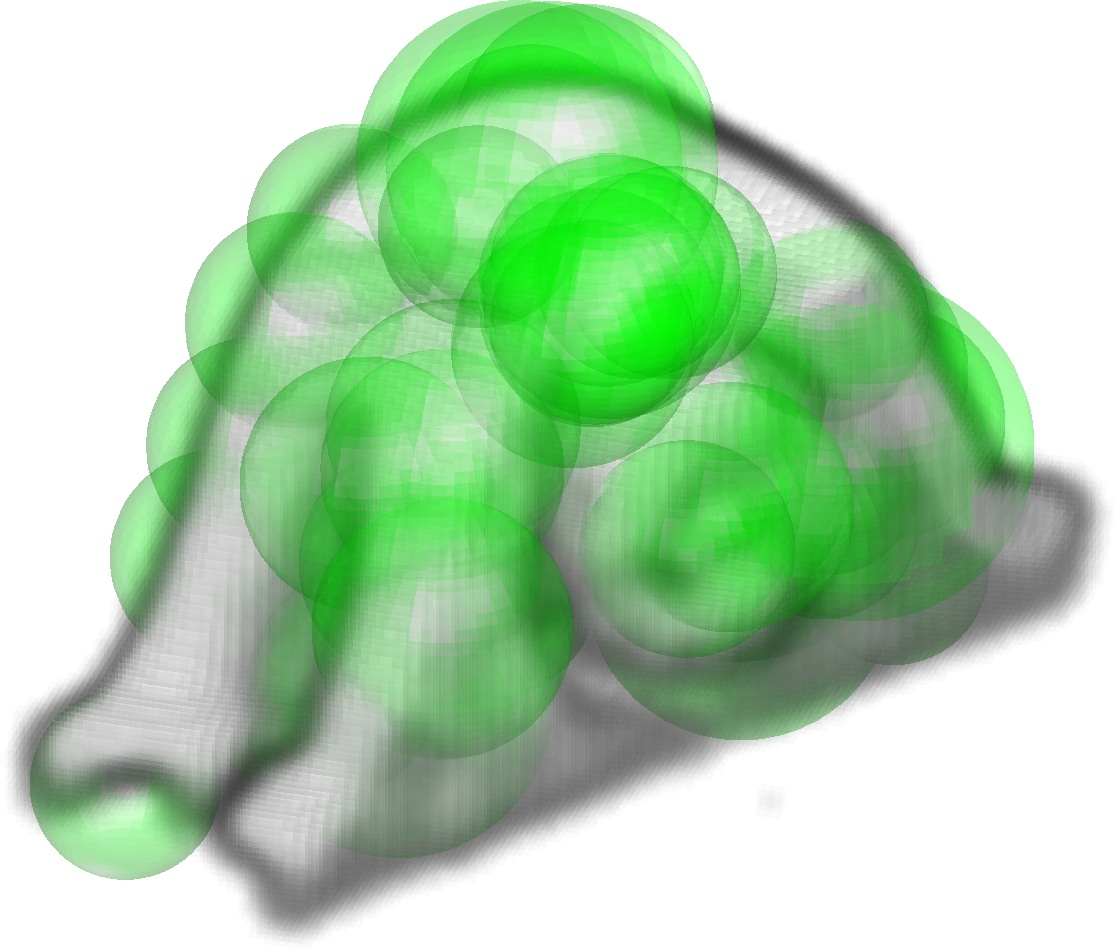
\includegraphics[width=0.175\linewidth]{./fig/eval/bearing_fast.jpg}  \hspace{0mm} 
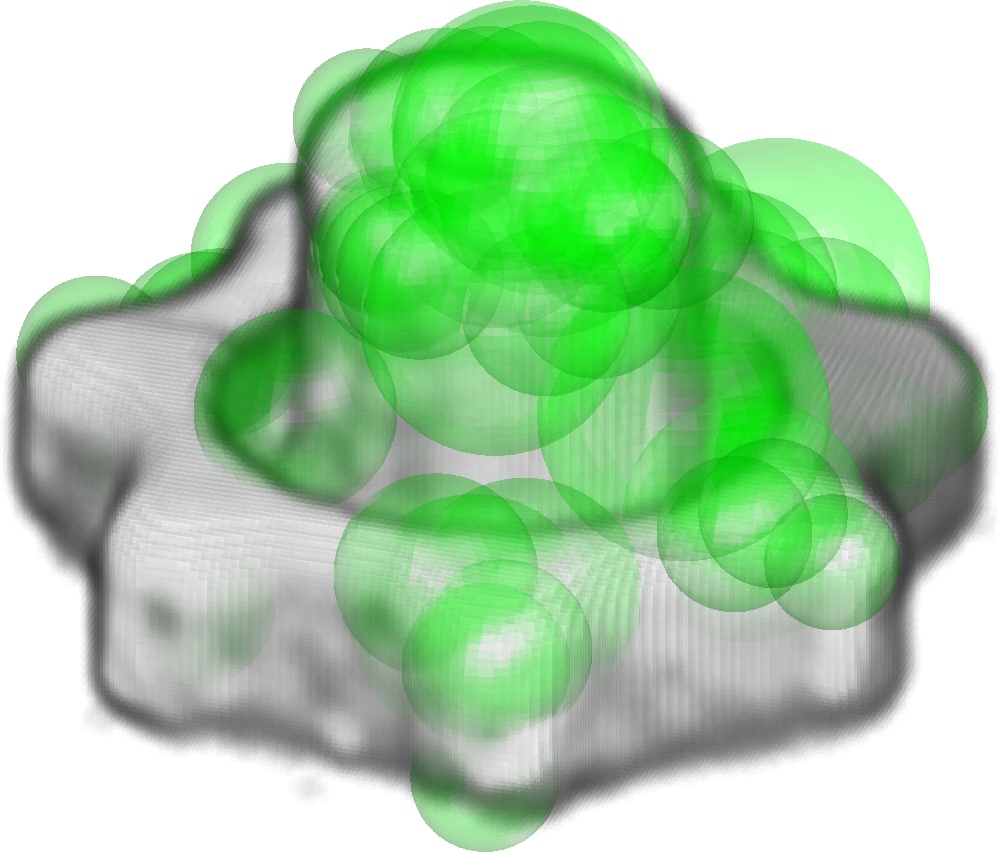
\includegraphics[width=0.175\linewidth]{./fig/eval/knob_fast.jpg} \hspace{0mm}
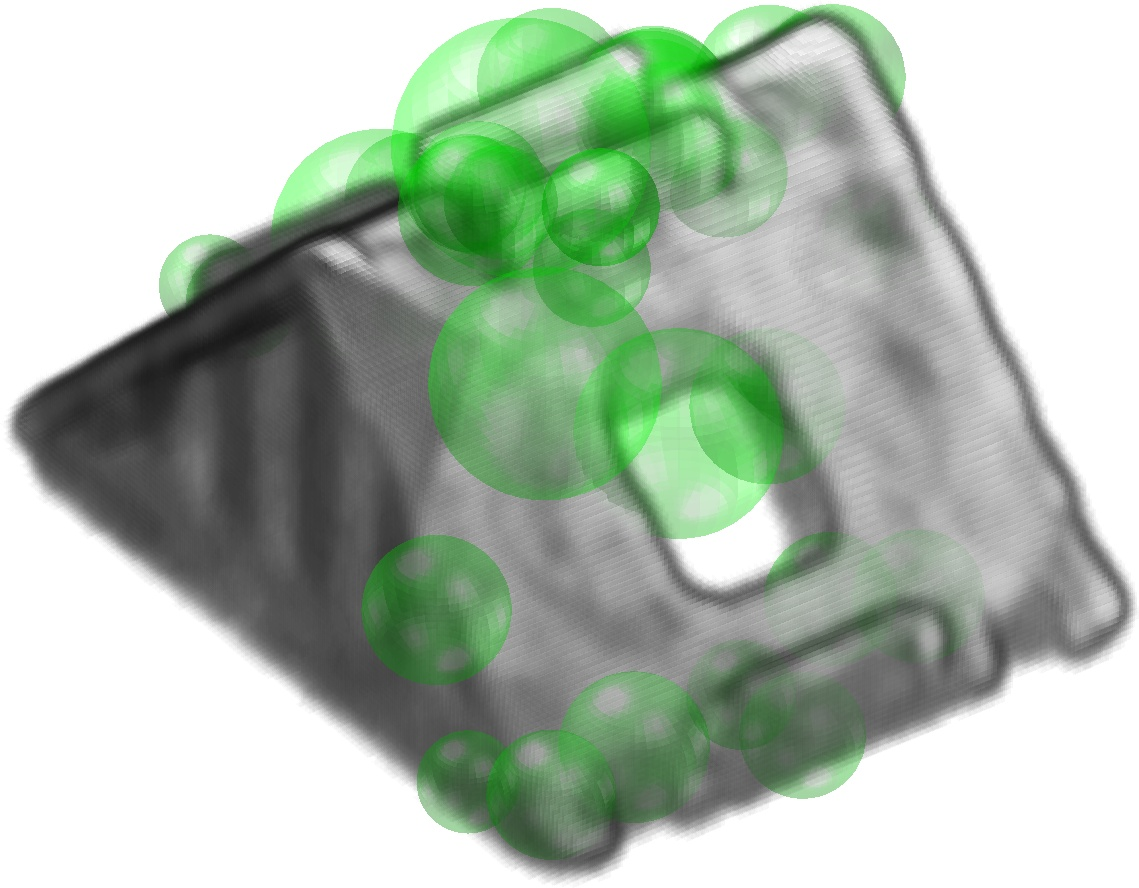
\includegraphics[width=0.175\linewidth]{./fig/eval/bracket_fast.jpg} 
} \vspace{-4.4mm}
\\
% MSER
\subfloat{ 
\label{fig:mvs:mser}
\makebox[0.15\linewidth]{\raisebox{0.07\linewidth}{(g) MSER}}
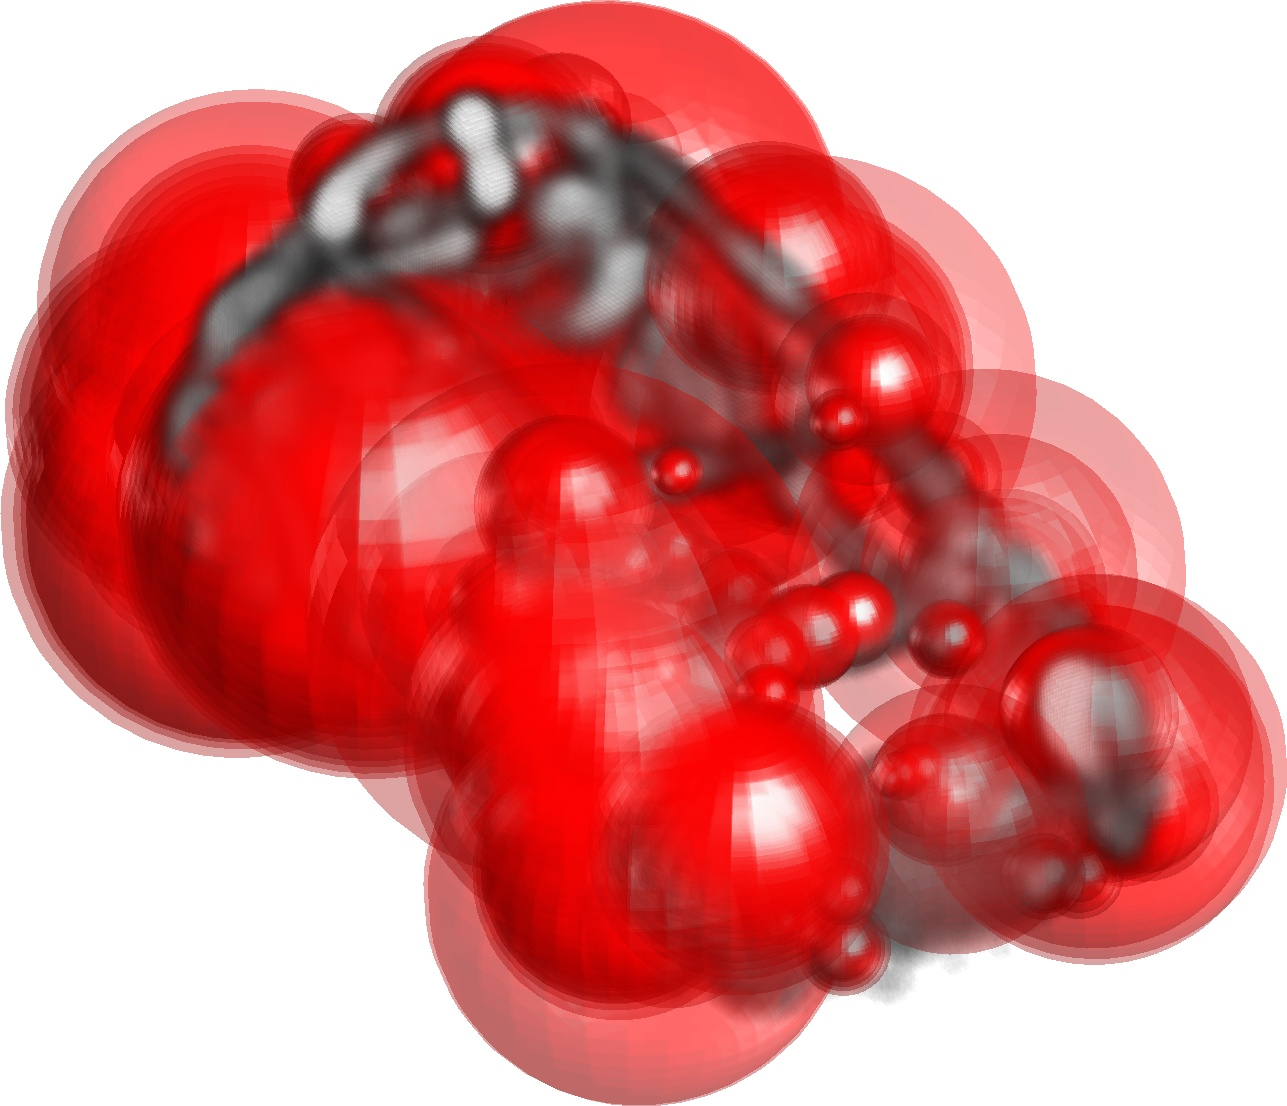
\includegraphics[width=0.175\linewidth]{./fig/eval/mini_mser.jpg} \hspace{0mm}
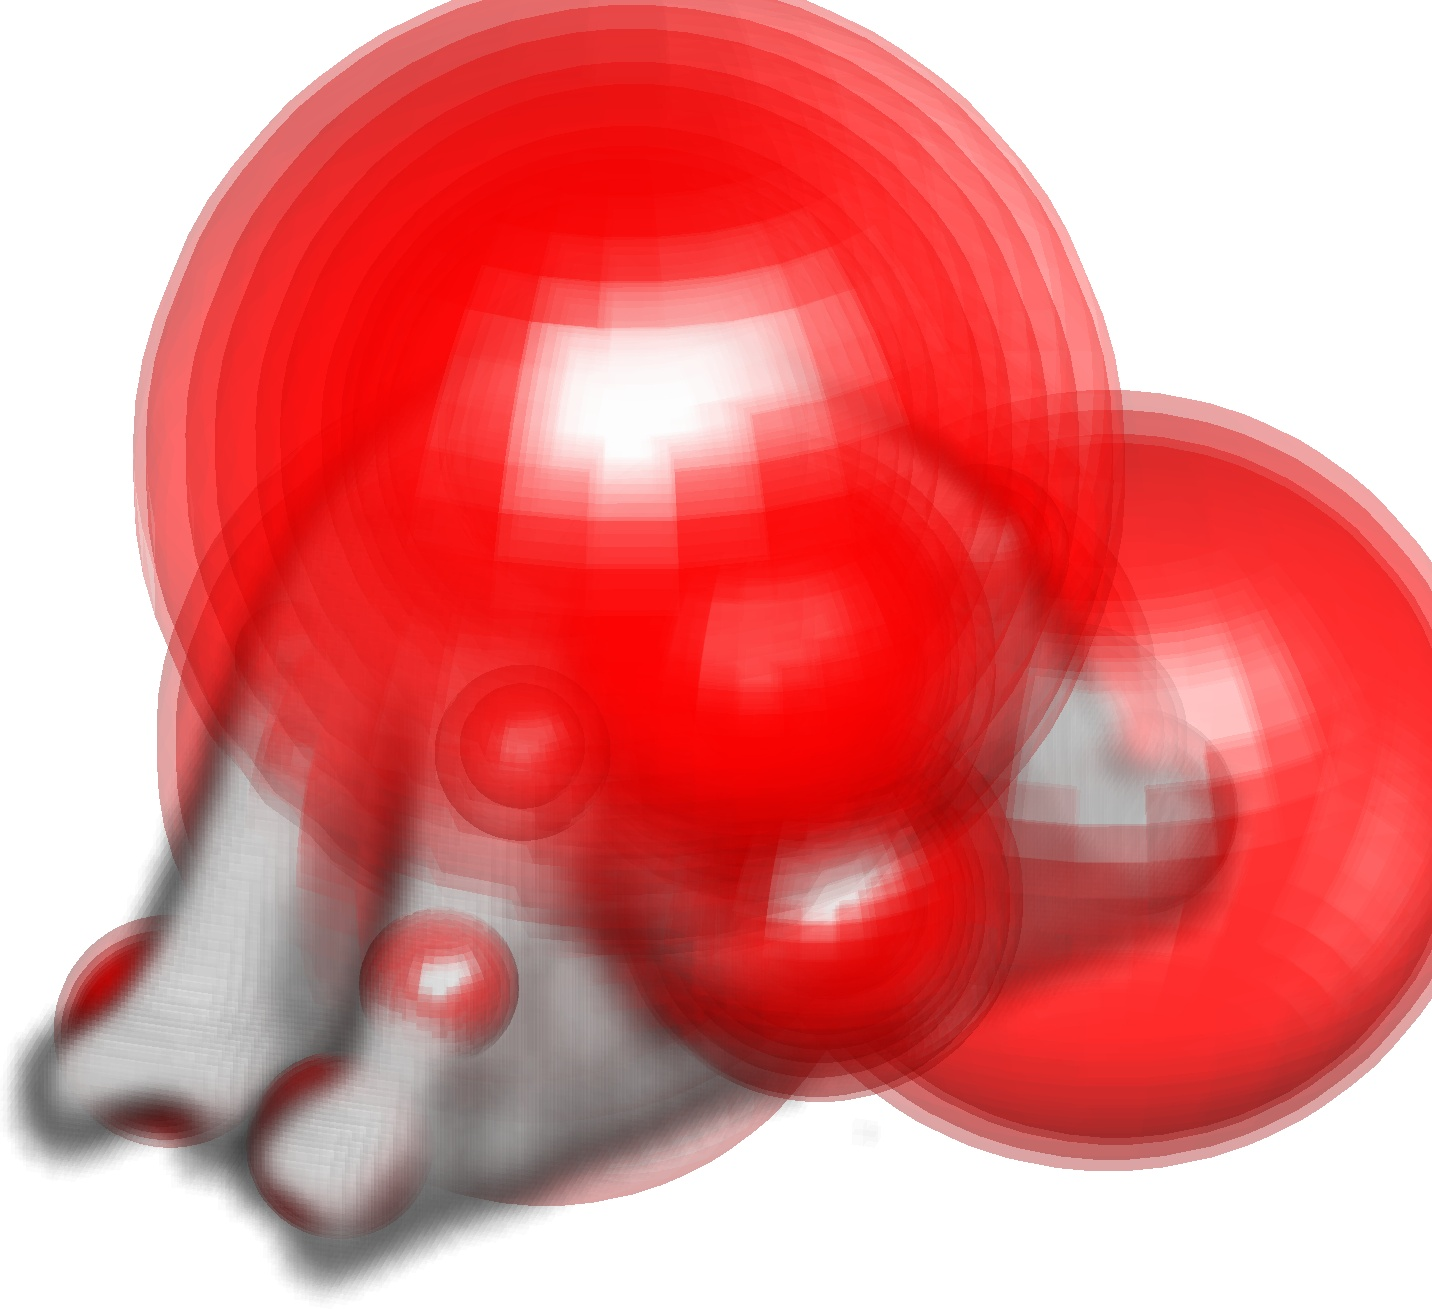
\includegraphics[width=0.175\linewidth]{./fig/eval/bearing_mser.jpg}  \hspace{0mm} 
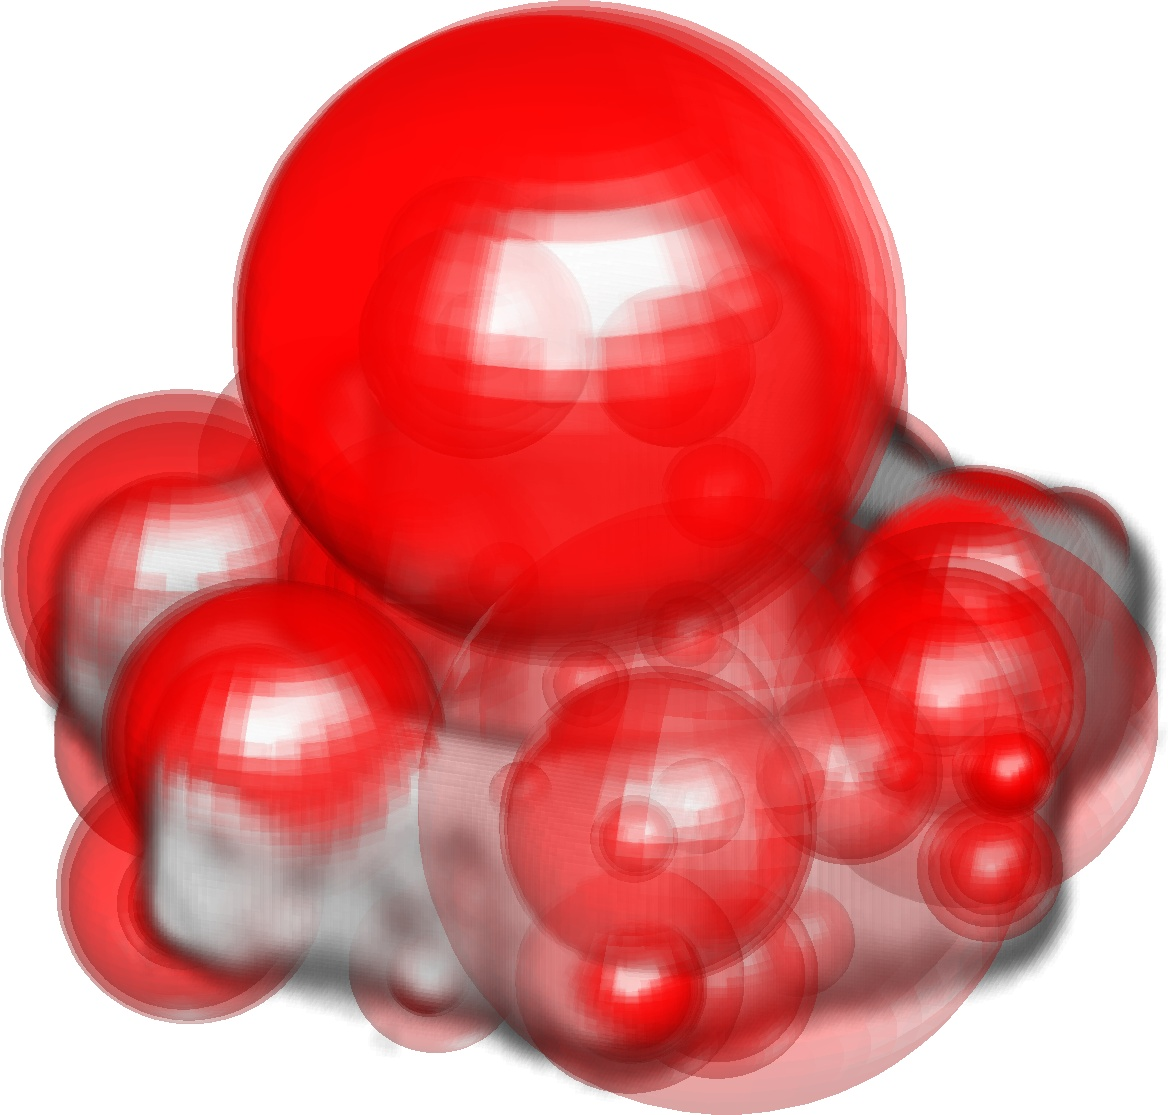
\includegraphics[width=0.175\linewidth]{./fig/eval/knob_mser.jpg} \hspace{0mm}
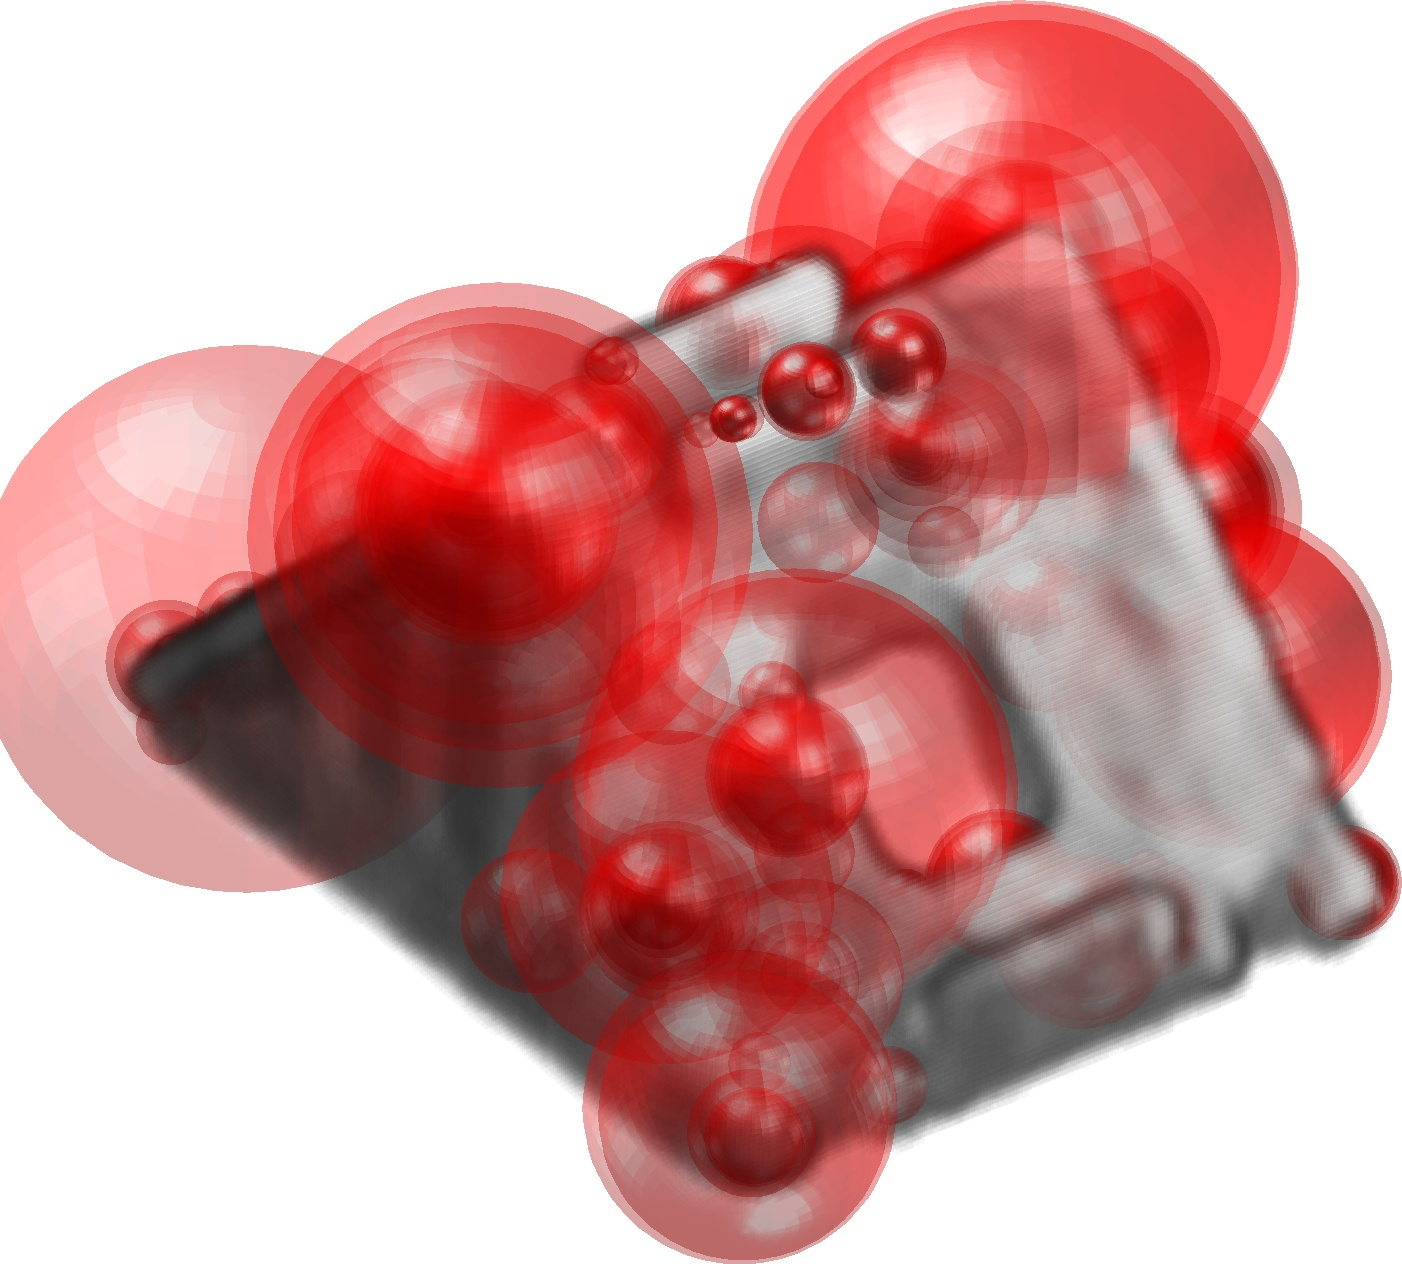
\includegraphics[width=0.175\linewidth]{./fig/eval/bracket_mser.jpg} 
} 
\caption{(a) Sample point clouds obtained from the \textbf{Stereo} dataset. (b) DoG, (c) SURF (d) Harris, (e) DoH, (f) V-FAST and (g) MSER interest points visualized on the voxelized data.}
\label{fig:mvs}
\end{figure*}
